\chapter{Models using Markov chains}
\label{chap:genetics}

\section{A simple genetic model}
The simplest type of genetic inheritance of traits in animals occurs when a certain trait is determined by a specific pair of genes, each of which may be two types, say $G$ and $g$. An individual may have a $GG$ combination, a $Gg$ (genetically equivalent to $gG$), or $gg$ combination. An individual with $GG$ is said to be dominant, a $gg$ individual is recessive and a $Gg$ is an hybrid.

In the mating of two animals, the offspring inherits one gene of the pair from each parent: the basic assumption of genetics is that these genes are selected at
random, independently of each other.


This assumption determines the probability
of occurrence of each type of offspring: The offspring
\begin{itemize}
\item of two dominant parents must be dominant, 
\item of two recessive parents must be recessive,
\item and of one dominant and one recessive parent must be hybrid.
\end{itemize}
In the mating of a dominant and a hybrid animal, each offspring must get a
$G$ gene from the former and has an equal chance of getting $G$ or $g$ from the latter.
Hence there is an equal probability of getting a dominant or a hybrid offspring.
Again, in the mating of a recessive and a hybrid, there is an even chance for getting
either a recessive or a hybrid. In the mating of two hybrids, the offspring has an
equal chance of getting $G$ or $g$ from each parent. Hence the probabilities are $1/4$
for $GG$, $1/2$ for $Gg$, and $1/4$ for $gg$.

A certain trait is determined by a specific pair of genes, each of which may be two types, say $G$ and $g$. 
One individual may have:
\begin{itemize}
\item $GG$ combination (\emph{dominant})
\item $Gg$ or $gG$, considered equivalent genetically (\emph{hybrid})
\item $gg$ combination (\emph{recessive})
\end{itemize}
In sexual reproduction, offspring inherit one gene of the pair from each parent. 


\subsection{Basic assumption of Mendelian genetics}
Genes inherited from each parent are selected at random, independently of each other.
This determines probability
of occurrence of each type of offspring. The offspring
\begin{itemize}
\item of two $GG$ parents must be $GG$, 
\item of two $gg$ parents must be $gg$,
\item of one $GG$ and one $gg$ parent must be $Gg$,
\item other cases must be examined in more detail.
\end{itemize}


\paragraph{$GG$ and $Gg$ parents}
\begin{center}
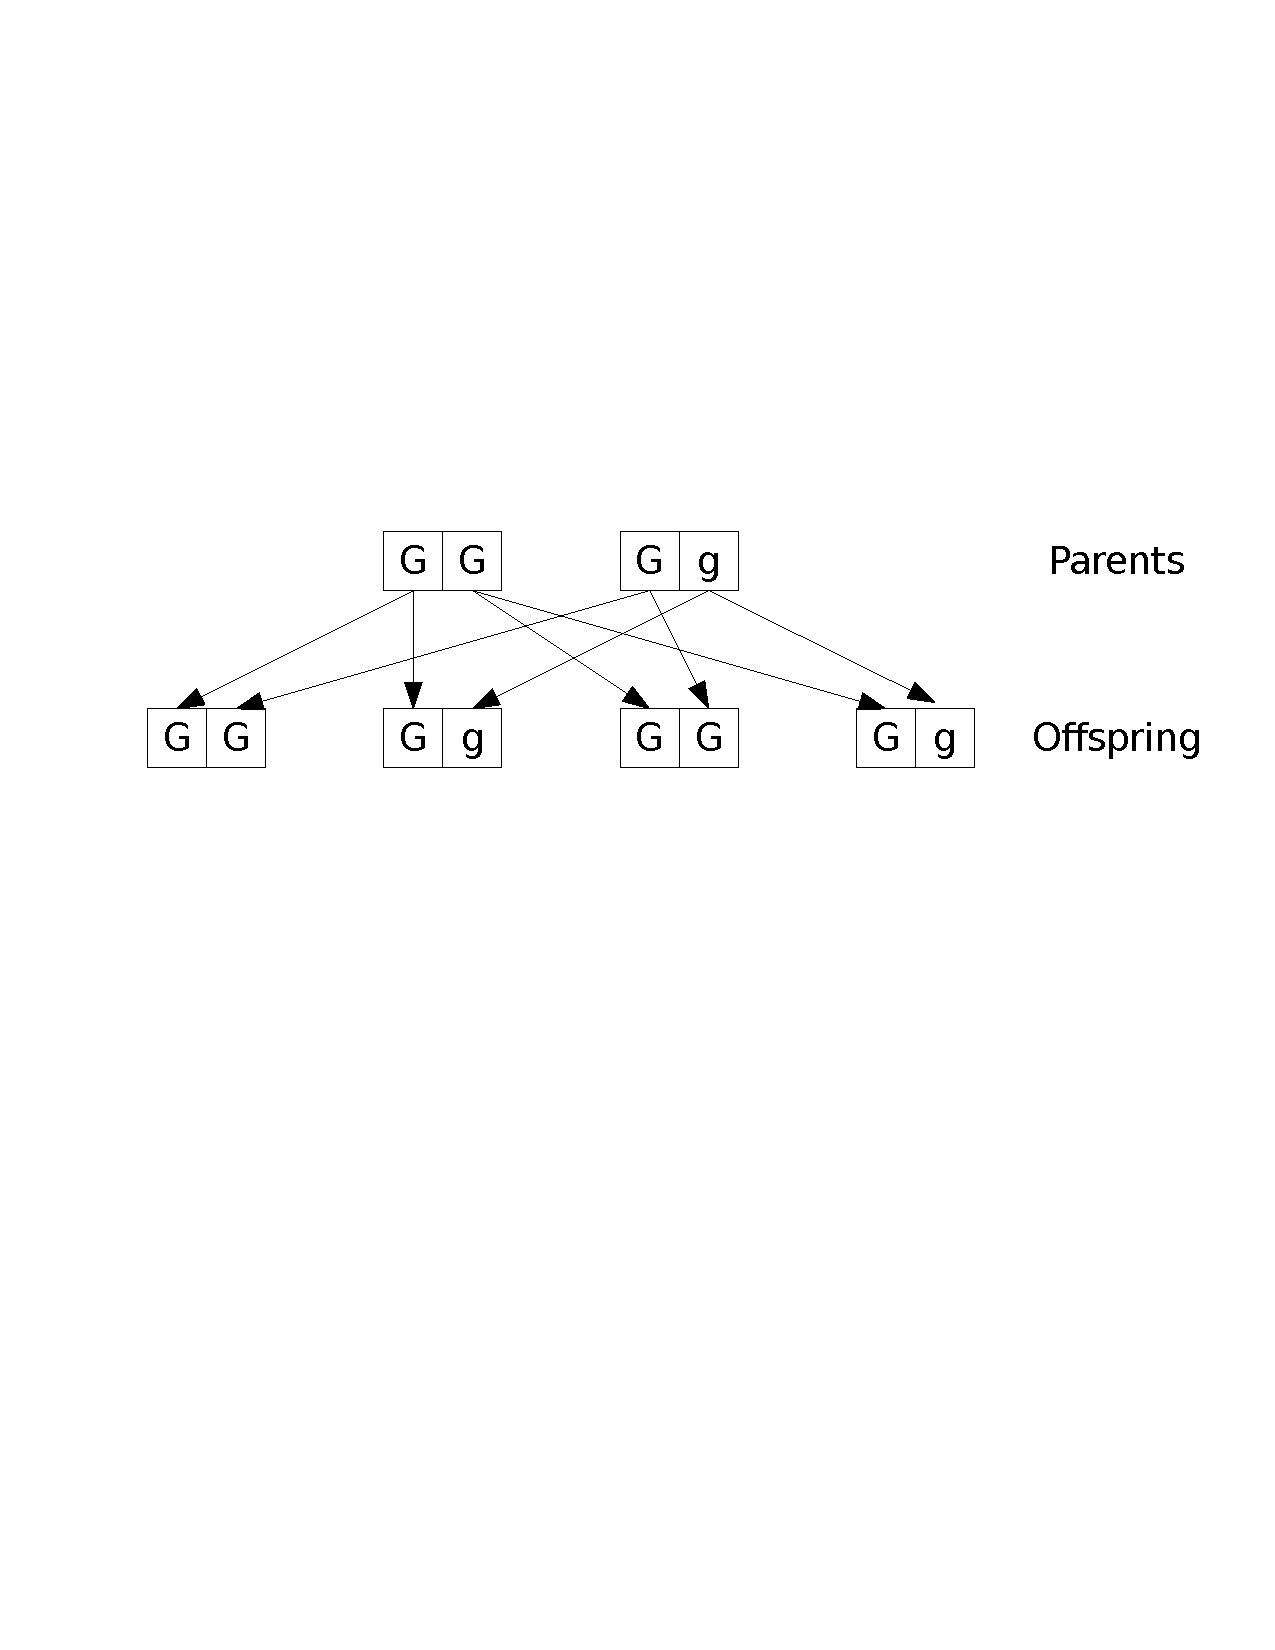
\includegraphics[width=0.5\textwidth]
{../figs_08_genetics/dominant_hybrid}
\end{center}
\vskip0.2cm
Offspring has probability $\dfrac 12$ of being $GG$ and $\dfrac 12$ of being $Gg$.

\paragraph{$Gg$ and $Gg$ parents}
\begin{center}
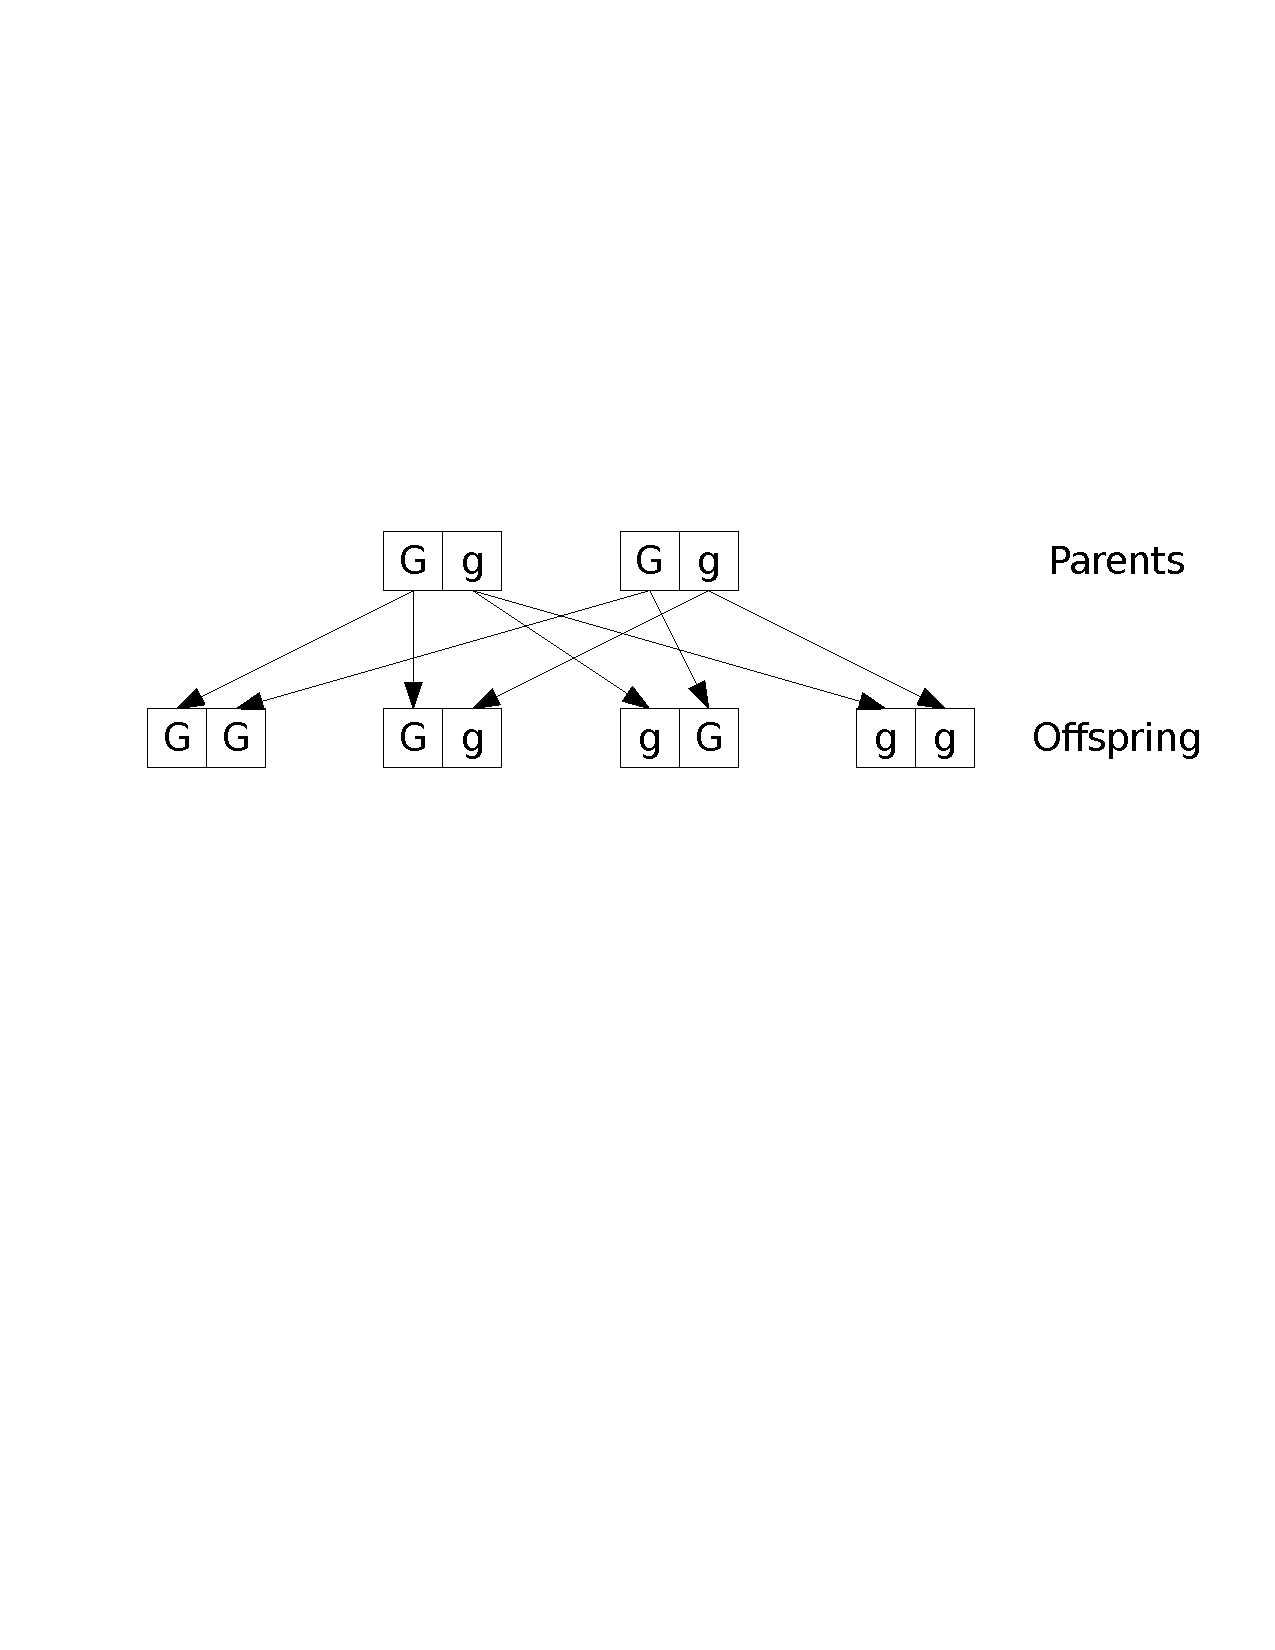
\includegraphics[width=0.5\textwidth]
{../figs_08_genetics/hybrid_hybrid}
\end{center}
\vskip0.2cm
Offspring has probability $\dfrac 14$ of being $GG$, $\dfrac 12$ of being $Gg$ and $\dfrac 14$ of being $gg$.


\paragraph{$gg$ and $Gg$ parents}
\begin{center}
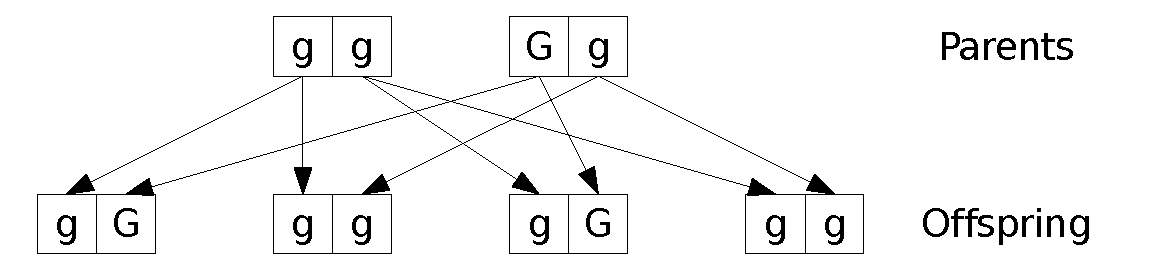
\includegraphics[width=0.5\textwidth]
{../figs_08_genetics/recessive_hybrid}
\end{center}
\vskip0.2cm
Offspring has probability $\dfrac 12$ of being $Gg$ and $\dfrac 12$ of being $gg$.


\subsection{A first genetic model -- Regular Markov chain}
Consider a process of continued matings with the following characteristics:
\begin{itemize}
\item Start with an individual of known or unknown
genetic character and mate it with a hybrid. 
\item Assume that there is at least one
offspring; choose one of them at random and mate it with a hybrid.
\item Repeat this process through a number of generations. 
\end{itemize}
The genetic type of the chosen
offspring in successive generations can be represented by a Markov chain, with states $GG$, $Gg$ and $gg$. So there are 3 possibles states $S_1=GG$, $S_2=Gg$ and $S_3=gg$.
We have
\begin{center}
\begin{tabular}{c|ccc}
$\nearrow$ & GG & Gg & gg \\
\hline
GG & 0.5 & 0.5 & 0 \\
Gg & 0.25 & 0.5 & 0.25 \\
gg & 0 & 0.5 & 0.5
\end{tabular}
\end{center}
The transition probabilities are thus
\[
P=\left (
\begin{array}{ccc}
\frac 12 & \frac 12 & 0 \\
\frac 14 & \frac 12 & \frac 14 \\
0 & \frac 12 & \frac 12
\end{array}\right).
\]
The (di)graph associated to $P$ is shown in Figure~\ref{fig:Markov_graph1}.
\begin{figure}[htbp]
\begin{center}
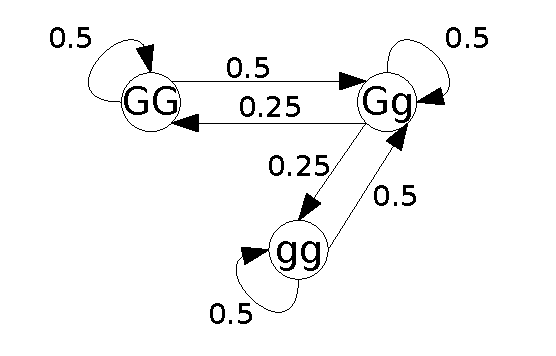
\includegraphics[width=0.5\textwidth]{../figs_08_genetics/graphe_hybride}
\caption{Transition graph for the Markov chain for the genetics model with mating with an hybrid individual.}
\label{fig:Markov_graph1}
\end{center}
\end{figure}
The Markov chain with transition matrix $P$ is regular. Indeed, compute $P^2$:
\[
P^2=\left (
\begin{array}{ccc}
\frac 38 & \frac 12 & \frac 18 \\
\frac 14 & \frac 12 & \frac 14 \\
\frac 18 & \frac 12 & \frac 38
\end{array}\right)
\]
As all entries are positive, $P$ is primitive and the Markov chain is regular. It is also possible to check this information directly by looking at the graph associated to the Markov chain (Figure~\ref{fig:Markov_graph1}). There, it is easy to check that it is possible to go from any state to any other state, i.e., the graph is strongly connected. From Theorem~\ref{th:connected_equiv_irreducible}, it follows that the matrix $P$ is irreducible. Further, the self-connecting loops mean that Theorem~\ref{} can be used, implying the primitivity of $P$.

Compute the left eigenvector associated to 1 by solving
\[
(w_1,w_2,w_3)
\left (
\begin{array}{ccc}
\frac 12 & \frac 12 & 0 \\
\frac 14 & \frac 12 & \frac 14 \\
0 & \frac 12 & \frac 12
\end{array}\right)=(w_1,w_2,w_3)
\]
\begin{subequations}
\begin{align}
\frac 12 w_1+\frac 14 w_2 &= w_1 \label{eq:l1} \\
\frac 12 w_1+\frac 12 w_2+\frac 12 w_3 &= w_2 \label{eq:l2} \\
\frac 14 w_2+\frac 12 w_3 &= w_3 \label{eq:l3} 
\end{align}
\end{subequations}
From \eqref{eq:l1}, $w_1=w_2/2$, and from \eqref{eq:l3}, $w_3=w_2/2$. Substituting these values into \eqref{eq:l2},
\[
\frac 14 w_2+\frac 12 w_2 +\frac 14 w_2=w_2,
\]
that is, $w_2=w_2$, i.e., $w_2$ can take any value. So $w=(\frac 14,\frac 12,\frac 14)$.



\subsection{A second genetic model -- Absorbing Markov chain}
Suppose now that we conduct the same experiment, but mate the individual picked at random in each new generation with a $GG$ individual instead of a $Gg$ individual. The transition table is
\begin{center}
\begin{tabular}{c|ccc}
$\nearrow$ & GG & Gg & gg \\
\hline
GG & 1 & 0 & 0 \\
Gg & 0.5 & 0.5 & 0 \\
gg & 0 & 1 & 0
\end{tabular}
\end{center}
and the resulting transition probabilities are
\[
P=\left (
\begin{array}{ccc}
1 & 0 & 0 \\
\frac 12 & \frac 12 & 0 \\
0 & 1 & 0
\end{array}\right)
\]

\begin{figure}[htbp]
\begin{center}
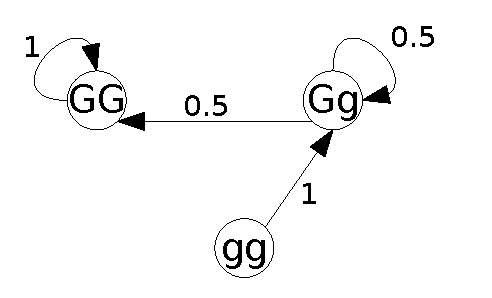
\includegraphics[width=0.45\textwidth]{../figs_08_genetics/graphe_dominant}
\caption{Transition digraph for the Markov chain for the genetics model with mating with a dominant individual. This graph is not strongly connected; vertex $GG$ is a \emph{sink}, while vertex $gg$ is a \emph{source}, or, in Markov chain vocabulary, state $GG$ is absorbing and state $gg$ is repulsive.}
\label{fig:Markov_graph2}
\end{center}
\end{figure}


Clearly,
\begin{itemize}
\item the process leaves $gg$ after one iteration, and can never return,
\item as soon as the process leaves $Gg$, it can never return there,
\item and it can never leave $GG$ as soon as it gets there.
\end{itemize}

The matrix is already in standard form,
\[
P=\left (
\begin{array}{ccc}
1 & 0 & 0 \\
\frac 12 & \frac 12 & 0 \\
0 & 1 & 0
\end{array}\right)
=\begin{pmatrix}
\mathbb{I}_1 & \mathbf{0} \\
R & Q
\end{pmatrix},
\]
with $\mathbb{I}_1=1$, $\mathbf{0}=(0\;\; 0)$ and
\[
R=\begin{pmatrix}
\frac 12\\ 0
\end{pmatrix}
\qquad
Q=\begin{pmatrix}
\frac 12 & 0\\
1 & 0
\end{pmatrix}.
\]
We have
\[
\mathbb{I}_2-Q=\begin{pmatrix}
1 & 0 \\
0 & 1
\end{pmatrix}
-\begin{pmatrix}
\frac 12 & 0\\
1 & 0
\end{pmatrix}
=\begin{pmatrix}
\frac 12 & 0\\
-1 & 1
\end{pmatrix},
\]
so
\[
N=(\mathbb{I}_2-Q)^{-1}=
2\begin{pmatrix}
1 & 0 \\
1 & \frac 12
\end{pmatrix}=
\begin{pmatrix}
2 & 0 \\
2 & 1
\end{pmatrix}.
\]
Then
\[
T=N\nbOne=\begin{pmatrix}
2\\
3
\end{pmatrix}
\]
and
\[
B=NR=
\begin{pmatrix}
2 & 0 \\
2 & 1
\end{pmatrix}
\begin{pmatrix}
\frac 12\\ 0
\end{pmatrix}
=
\begin{pmatrix}
1\\ 1
\end{pmatrix}.
\]